\documentclass[]{article}
\usepackage{caption,subcaption,graphicx,float,url,amsmath,amssymb,amsthm,tocloft,cancel,thmtools,gensymb,braket}
\usepackage[toc,nonumberlist]{glossaries}
\usepackage{glossaries-extra}
\newcommand\numberthis{\addtocounter{equation}{1}\tag{\theequation}}

\newtheorem{thm}{Theorem}
\newtheorem{defn}[thm]{Definition}
\newtheorem{cor}[thm]{Corollary}
\newtheorem{lemma}[thm]{Lemma}
\graphicspath{{figs/}}
\widowpenalty10000
\clubpenalty10000
\setcounter{tocdepth}{1}

%opening
\title{Theoretical Minimum\\Particle Physics 1\\Basic Concepts}
\author{Simon Crase(compiler)}

\begin{document}

\maketitle

\begin{abstract}
These are my notes for Particle Physics 1 lectures from Leonard Susskind's Theoretical Minimum series.
\end{abstract}

\tableofcontents
\listoffigures
\listoftheorems

\section{Particles and Light}

This lecture contains  facts from other courses, which will be used on later lectures.

Particle physics is about the question: is matter discrete? If so we will call the smallest things "particles". If matter forms a continuum, we have fields.

Which is correct? Both and neither.

First evidence for atoms came from chemistry. John Dalton looked at mass mole: each substance was an integer multiple of mass of a mole of hydrogen; it suggested that there are building blocks. We now know that mass of molecule is mass of protons, electrons (very small), and neutrons, which have nearly the same mass as protons. 
 
Figure \ref{fig:em:wave} illustrates an electromagnetic wave. We need the concepts of wavelength, $\lambda$, and period, $T$.

We have
\begin{align*}
\frac{\lambda}{T}=&c\\
f=&\frac{1}{T} \text{, so}\\
\lambda f =& c\text{. Physicists tend to measure frequency in radians per second:}\\
\omega =& 2 \pi f \text{, so} \\
\omega =& \frac{2 \pi c}{\lambda} \numberthis \label{eq:omega:lambda}
\end{align*}

\begin{figure}[H]
	\caption{An electromagnetic wave}\label{fig:em:wave}  
	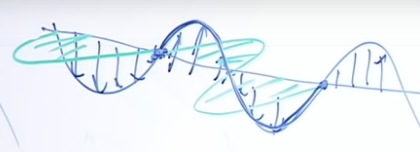
\includegraphics[width=0.9\textwidth]{Wavelength}
\end{figure}

Wave/particle duality.

A photon has energy:
\begin{align*}
E=&\hslash \omega \text{. Energy of single photon.} \numberthis\label{eq:E_omega}\\
E_{ray}=&n \hslash \omega \text{. Energy of ray.}
\end{align*}
 

In modern usage, mass is what used to be called rest mass. $E = m c^2$ only for stationary object.

In particle physics we choose units to set $c=1$ and $\hslash=1$. In this lecture $c$ and $\hslash$ will appear explicitly only when Prof. Susskind wants to show the magnitude of some quantity.

Energy depends on the motion of the object as seen by the observer: it isn't a universal thing that everyone will agree on.

Light has energy and momentum (not mass): 

\begin{align*}
\left|P\right|=&\frac{E}{c} \\
=&\frac{\hslash \omega}{c} \text{, from (\ref{eq:E_omega})}\\
=& \frac{2 \pi \hslash}{\lambda} \text{, from (\ref{eq:omega:lambda}). c.f. Harmonic Oscillator.}\numberthis\label{eq:P:lambda}
\end{align*}

This is why we need larger and larger instruments to observe smaller particles!
To see really small things, we need particles with high energy and momentum.


\section{Quantum field theory}

\subsection{Mathematical Preliminaries}

Consider a classical wave $A \sin(kx)$. Energy is $A^2$, but it is also proportional to number of photons, $n$: $E \propto n \hslash \omega$, $A \propto \sqrt(n)$.

Generally, equations containing $c$ apply for photons only. For non-relativistic particles:
\begin{align*}
E=&\frac{p^2}{2m}\\
f =& \frac{h}{2 m \lambda^2} \text{. c.f. Schr\"odinger equation!}
\end{align*}

\begin{itemize}
	\item Phase Velocity: velocity of wave packet;
	\item Group velocity: velocity of troughs and peaks--identified with particle velocity.
\end{itemize}

For light waves, phase and group velocities the same, but this isn't true for most particles. Phase velocity can exceed $c$, but can't transmit information.

Space is infinite. But physics is the art of getting problems into a shape that computers can solve, so we need to remove infinities.

Let's look at 1 dimensional waves. We can restrict to fixed length $L$: reflecting boundary condition at ends. But this violates conservation of momentum. Instead use a topological "circle" circumference $L$--periodic boundary conditions. As a consequence momentum is quantized: 

\begin{align*}
\lambda =& \frac{L}{N}\\
P =& \frac{h}{\lambda}\\
=& \frac{h N}{L}
\end{align*}

Now make into a real circle, radius $R$, and redefine $L$ to be \emph{angular momentum}.

\begin{align*}
P =& \frac{h N}{2 \pi R}\\
L =& N \frac{h}{2 \pi}\\
=& N \hslash \text{ independent of $R$.}
\end{align*}

\subsection{Quantum field theory}

Start with harmonic oscillator: a wave is a collection of harmonic oscillators. Energy is quantized: 0, $\hslash \omega$, $2\hslash \omega$...

Introduce operators:

\begin{align*}
a^+ \ket{n} =& \sqrt{n+1} \ket{n+1} \text{, creation operator}\\
a^- \ket{n} =& \sqrt{n} \ket{n-1} \text{, annihilation operator}\\
a^+ a^- \ket{n} =& n \ket{n} \text{, or}\\
a^+ a^-  =& n \text{, similarly}\\
a^- a^+  =& n+1\\
[a^-, a^+] =& 1
\end{align*}

Return to world on a circle--$\omega_N$--equivalent to oscillator. State is $\ket{n_1,n_2, n_3,...}$--occupation numbers. 
\begin{defn}[quantum field]
	A quantum field is a collection of harmonic oscillators, togther with annihilation operators and creation operators.
\end{defn}

\section{Quantum fields and particles}

\section{More quantum field theory}

\section{Energy conservation and waves}

\section{Dirac equation and Higgs particles}

\section{Angular momentum}

\section{Spin}

\section{Equations of motion of particles and fields}

\section{Field Lagrangians and path integrals}


\end{document}
